%!TEX root = ../thesis.tex
%*******************************************************************************
%*********************************** First Chapter *****************************
%*******************************************************************************

\chapter{Introduction} %Title of the First Chapter

\ifpdf
    \graphicspath{{Chapter1/Figs/Raster/}{Chapter1/Figs/PDF/}{Chapter1/Figs/}}
\else
    \graphicspath{{Chapter1/Figs/Vector/}{Chapter1/Figs/}}
\fi


%********************************** %First Section  **************************************
\section{Background} %Section - 1.1 

% \textbf{Thesis statement: studying evolutionarily basal organisms lets us study the simple ways that nature exploits geometry in living systems without higher order functional complications.}

\begin{comment}

\nomenclature[z-cif]{$CIF$}{Cauchy's Integral Formula}                                % first letter Z is for Acronyms 
\nomenclature[a-F]{$F$}{complex function}                                                   % first letter A is for Roman symbols
\nomenclature[g-p]{$\pi$}{ $\simeq 3.14\ldots$}                                             % first letter G is for Greek Symbols
\nomenclature[g-i]{$\iota$}{unit imaginary number $\sqrt{-1}$}                      % first letter G is for Greek Symbols
\nomenclature[g-g]{$\gamma$}{a simply closed curve on a complex plane}  % first letter G is for Greek Symbols
\nomenclature[x-i]{$\oint_\gamma$}{integration around a curve $\gamma$} % first letter X is for Other Symbols
\nomenclature[r-j]{$j$}{superscript index}                                                       % first letter R is for superscripts
\nomenclature[s-0]{$0$}{subscript index}                                                        % first letter S is for subscripts
\end{comment}

Discuss evolutionary origins of multicellularity and some basic examples like Volvox. What drives organisms to become multicellular? 
We expect there was genuine evolutionary favorability to developing multicellularity. 
In the volvocine algae, it is believed that the transition to multicellularity and cooperation of distinct differentiated cells has occured several times \citep{herron2008}. 
Across all eukaryotic lineages, there is evidence that multicellularity evolved independently many times \citep{king2004}.

Organisms like vovocine green algae and choanoflagellates are sought as models in the search for evolutionary origins of multicellularity for both their biological and physical features \citep{goldstein2015}. 
Choanoflagellates have long been regarded as a close relative to the animal kingdom owing to their similarity to choanocytes in sponges \citep{james1871}, and we now understand them to be most closely related by genetics \citep{lang2002,sebe2017}.
These organisms' colonies are also large enough that they operate at high P\'eclet number ($Pe \sim 10^2$), the ratio between advective and diffusive transport, meaning that advection must contribute substantially to deriving food \citep{solari2006}. 
This of course contrasts with typical bacteria, where diffusion dominates nutrient transport \citep{berg1977}.

\subsection{Why attach?} % ** Why attach?

\mynote{could probably say some stuff about bacteria and biofilms here}

From a simplistic optimality perspective, we do not readily identify a motivation for attaching. 
\citet{michelin2011} demonstrated that regardless of P\'eclet number, cells feed optimally when they maximise their swimming velocity. 
Despite this solution, \citet{kirkegaard2016} modeled for cell arrangements such as the choanoflagellate colonies to be studied in this work (\cref{sec:choano}) that swimming is maximised for individual cells. 
When collared choanoflagellates are near each other, cells with their flagella pointing in the same direction (\textit{i.e.} a straight chain) are best at swimming.
Based on feeding efficiency via swimming alone, it does not appear that basic aquatic multicellular colonies, such as \textit{S. rosetta} or \textit{C. flexa} have much to gain from their propulsion cooperation.

The organisms in the \textit{Volvox} genus are well studied for being a primitive example of multicellularity and a shining beacon of functional geometric changes. 
These organisms attach their cells to one another using an extra-cellular matrix, as \textit{S. rosetta} does as well (discussed later). 

One suggestion for cell-cell attachment in colonies is to avoid phagocytosis from predators by physically becoming too large. 
\citet{stanley1973} argues that the emergence of heterotrophs, or organisms that derive energy by consuming others, led to rapid diversification and the rise of multicellularity through intense selective pressure. 
\citet{boraas1998} demonstrated in a laboratory culture that stable multicellularity emerged in the green alga \textit{Chlorella vulgaris} when exposed to predators.
Eight-cell colonies were observed to predominate, indicating that multicellularity emerged to balance colony survival as well as individual demands of each cell.

% * Attaching supports flows

\subsubsection*{Attaching supports generating flows}
Spherical colony geometries have long been documented \citep{lauterborn1898} for choanoflagellates. 

We understand, for example, in \textit{Volvox} colonies that driving flows supports nutrient transport by advection as well as phototaxis. 

\mynote{Here is a good place to describe sponges!}

% ** Why differentiate?
\subsection{Why differentiate?}

We are interested in multicellularity at an evolutionarilty basal level to understand the basic reasons that life evolved to form multicellular organisms. Sponges are as basal as multicellular animal life goes \mynote{Discuss why and reference a review about sponges evolutionary simplicity. \citet{carr2008} could be a good ref to give here regarding choanoflagellates}. 

\mynote{discuss \citet{dayel2011} about differentiation in \textit{S. rosetta}}

While we are interested in sponges since they are members of the animal kingdom, choanoflagellates are often considered to be evolutionarily and morphologically comparable. 



%********************************** %Second Section  *************************************
\section{Choanoflagellates} \label{sec:choano} %Section - 1.2 

\mynote{Discuss \citet{carr2008} about molecular phylogeny of choanoflagellates}

The connection between choanoflagellates and animals predates studies using molecular phylogeny. 
\citet{james1871} first compared choanoflagellate morphology with the choanocytes in sponge choanocyte chamber. 
Morphological similarities between choanocytes and protists led to the belief that the two emerged from a common ancestor \citep{saedeleer1930,tuzet1963}.

\citet{mah2014} offers the first comprehensive comparison between sponge choanocyte and choanoflagellate morphology. Sponge collars are fairly cylindrical while choanoflagellate collars are more cone-like. Choanoflagellates have glycocalyx, but seemingly around the cell body \citep{leadbeater2008}. Notably the collars in choanoflagellates are always microvillar and always present, while in sponges they emerge as a consequence of cell differentiation \mynote{cite this!}. 

Choanoflagellates are increasingly studied as a model for understanding how multicellular animal life emerged. \citet{fairclough2010} shows that the transition from single cell to multicellular colony in \textit{Salpingoeca rosetta} occurs by cell division, with cells remaining attached to each other. 

\textit{S. rosetta} has an extracellular matrix \citep{larson2020}. \citet{larson2020} finds that the extracellular matrix constrains cells to grow and divide to a given colony shape. This paper also finds that \textit{S. rosetta} does not have distinct cell lineages or a developmental plan.

\citet{kirkegaard2016} finds that collared choanoflagellates drive the most flow through their collars by swimming fastest, which occurs in the unicellular state \citep{michelin2011}. This makes it unclear that forming rosette colonies is for the sake of improved feeding. The authors point to evidence that \textit{S. rosetta} is induced to form rosette colonies by bacterial cues to suggest that the reasons for the development of multicellularity may be more subtle than previously expected \citep{alegado2012}.

%********************************** % Third Section  *************************************
\section{\textit{Choanoeca flexa}}  %Section - 1.3 

% intro`
\citet{brunet2019} describe a newly discovered choanoflagellate, \textit{Choanoeca flexa}, which lives and feeds in aquatic environments. 
Here, I describe the relevant properties and characteristics of these cells and their colonies for modeling its structure and behavior. 
All descriptions of \textit{C. flexa} proceed from \citet{brunet2019} and private communications with the authors.

% general description
\textit{C. flexa} is an aquatic colonial choanoflagellate that forms sheets on the order of $\SI{100}{\micro\meter}$ in diameter (\cref{fig:cflexa}).
Each cell in a colony consists of a cell body ($\sim \SI{4}{\micro\meter}$), microvillar collar ($\sim\SI{10}{\micro\meter}$ length), and apical flagellum at the collar centre.
All observed sheets have had flagella facing in the same direction, giving the sheet two distinct sides.
Cells attach to each other through their collar microvilli, and in contrast to a colonial flagellate like \textit{S. rosetta}, there is no evidence for an extracellular matrix holding cells together in \textit{Choanoeca} \citep{leadbeater1983,brunet2019}.
Collar microvilli are distinct and colony cells demonstrated no intercellular cytoplasmic bridges (contrast with \textit{i.e. Volvox}), with cells detaching from each other upon treatment with calcium \citep{thibaut}.
\mynote{double check that it was calcium!}
By comparison with division in \textit{C. perplexa}, colony cells are expected to undergo cell division with temporary incomplete replication, where the pair of daughter cells is attached by some shared collar microvilli (\cref{fig:division}).
Colonies are believed to occasionally fragment to separate completely and multiply \citep{leadbeater1983}.

% thecate and division
\textit{C. flexa} also exhibits a sedentary, unicellular form that adheres to surfaces via a stalk (\textit{theca}) without a flagellum, as in \textit{C. perplexa}.
Our understanding of cell division in \textit{Choanoeca} emerges from the thecate form, which leaves one thecate daughter cell and another motile, flagellated cell.
Division begins with the generation of a flagellum by the thecate cell and proceed with protoplasm division with incomplete separation at collar microvilli (\cref{fig:division}) \citep{ellis1930,leadbeater1977}.
The remainder of this work concerns the colonial form of \textit{C. flexa} rather than the thecate or unicellular motile forms.
While we do not have observations on cell replication in the colonial phase, \textit{S. rosetta} gives a suggestion that colonial choanoflagellates do not coordinate their cell division \citep{fairclough2010}.

\begin{figure}[htbp]
	\centering
	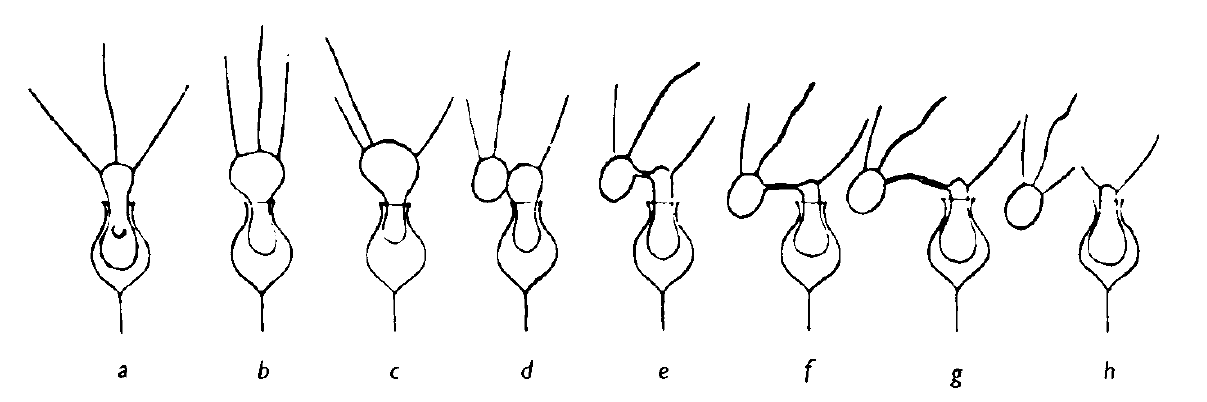
\includegraphics[width=\textwidth]{division.png}
	\caption[Illustrations of stages of division in the sessile form of \textit{C. perplexa}]{Illustrations of stages of division in the sessile form of \textit{C. perplexa}. Reproduced from \citet{leadbeater1977} based on \citet{ellis1930} with permission from Cambridge University Press.}
	\label{fig:division}
\end{figure}

While choanoflagellate colonies typically orient their flagella to point away from the colony centre, sheets of \textit{Choanoeca} in their rest state point flagella inward. \mynote{cite this! \citet{brunet2019} uses a leadbeater textbook}

\subsection{Sheet inversion}

% inversion introduction
\textit{Choanoeca} has recently sparked renewed interest as a result of the characterisation of rapid light-regulated inversion in colonies, which causes cell sheets to change orientation from pointing flagella-in to flagella-out \citep{brunet2019}.
The inversion is understood to result from contraction of an actomyosin ring at the apical end of colony cells, which results in collar microvilli flaring out. 
This result is consistent with a description of conraction the cell apex with changes in collar angle for \textit{C. perplexa} cells \citep{leadbeater1977}.
Sheet inversion takes $\sim\SI{10}{\second}$.
Notably, deviations in \textit{C. perplexa} collar angle (between $10^\circ-90^\circ$ from the apicobasal axis) were described in \citet{ellis1930}, and \citet{leadbeater1983} described colonies now understood to be \textit{C. perplexa} undergoing inversion. 
\footnote{The latter attributes inversion to a reversal of flagellum rotation, though this explanation is unlikely given the more recent evidence for \textit{C. flexa} \citep{brunet2019}.}
Collar stiffness and the intrinsic curvature in collars facilitates a clear preference in sheet curvature. 
Collars in thecate cells have been described as flaccid \citep{leadbeater1977}, suggesting that an increase in collar stiffness is essential to the transition to colony-forming cells. 

% describing two states
\citet{brunet2019} identified several factors that contribute or prohibit sheet inversion. 
It is believed that, in their natural environment, sheet inversion from flagella-in to flagella-out is triggered by darkness. 
In the inverted (flagella-out) state that occurs in darkness, individual cells demonstrated contraction of an apical actomyosin ring.
The contraction results in collar microvilli flaring out: relative to the apicobasal axis measured at the base of the flagellum, the median collar microvillus angle moved out from $\sim35^\circ$ to $\sim50^\circ$.
This increase in angle is largely the result of collar microvilli straightening out: in light, single colony-cells' collars curve to align with the apicobasal axis after emerging from the apical ends of cells.
\mynote{add figure of individual cells}
Cell sheet area decreases significantly since cell bodies are in contact in the inverted state \citep{thibaut}.
These properties are summarised in \cref{subfig:table}.

% what does inversion achieve?
The transition to the flagella-out state results in a significant increase in swimming speed \citep{brunet2019}. 
In contrast, flagella-in sheets are non-motile to the extent that they typically sink. 
The lack of mobility is compensated by an increase in cells phagocytosed by several times: flagella-in sheets are substantially more effective at driving flow towards the collars, where individual cells feed.
Increased motility in the dark-induced state and accumulation in regions with light facilitates a primitive form of phototaxis.
\mynote{why does swimming not directly translate to feeding as in lauga2011 paper?}

\begin{figure}[htbp]
	\centering
	\begin{subfigure}[b]{0.7\textwidth}
		\centering
		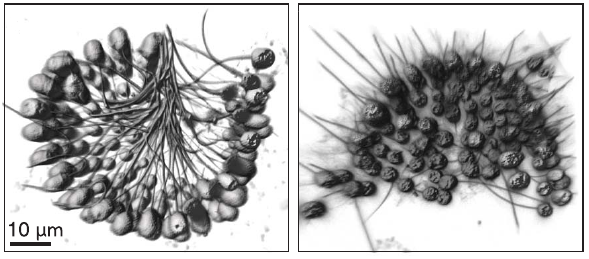
\includegraphics[width=\textwidth]{cflexa.png}
		\caption{}
		\label{subfig:cflexa}
	\end{subfigure}
	\begin{subfigure}[b]{0.29\textwidth}
		\centering
		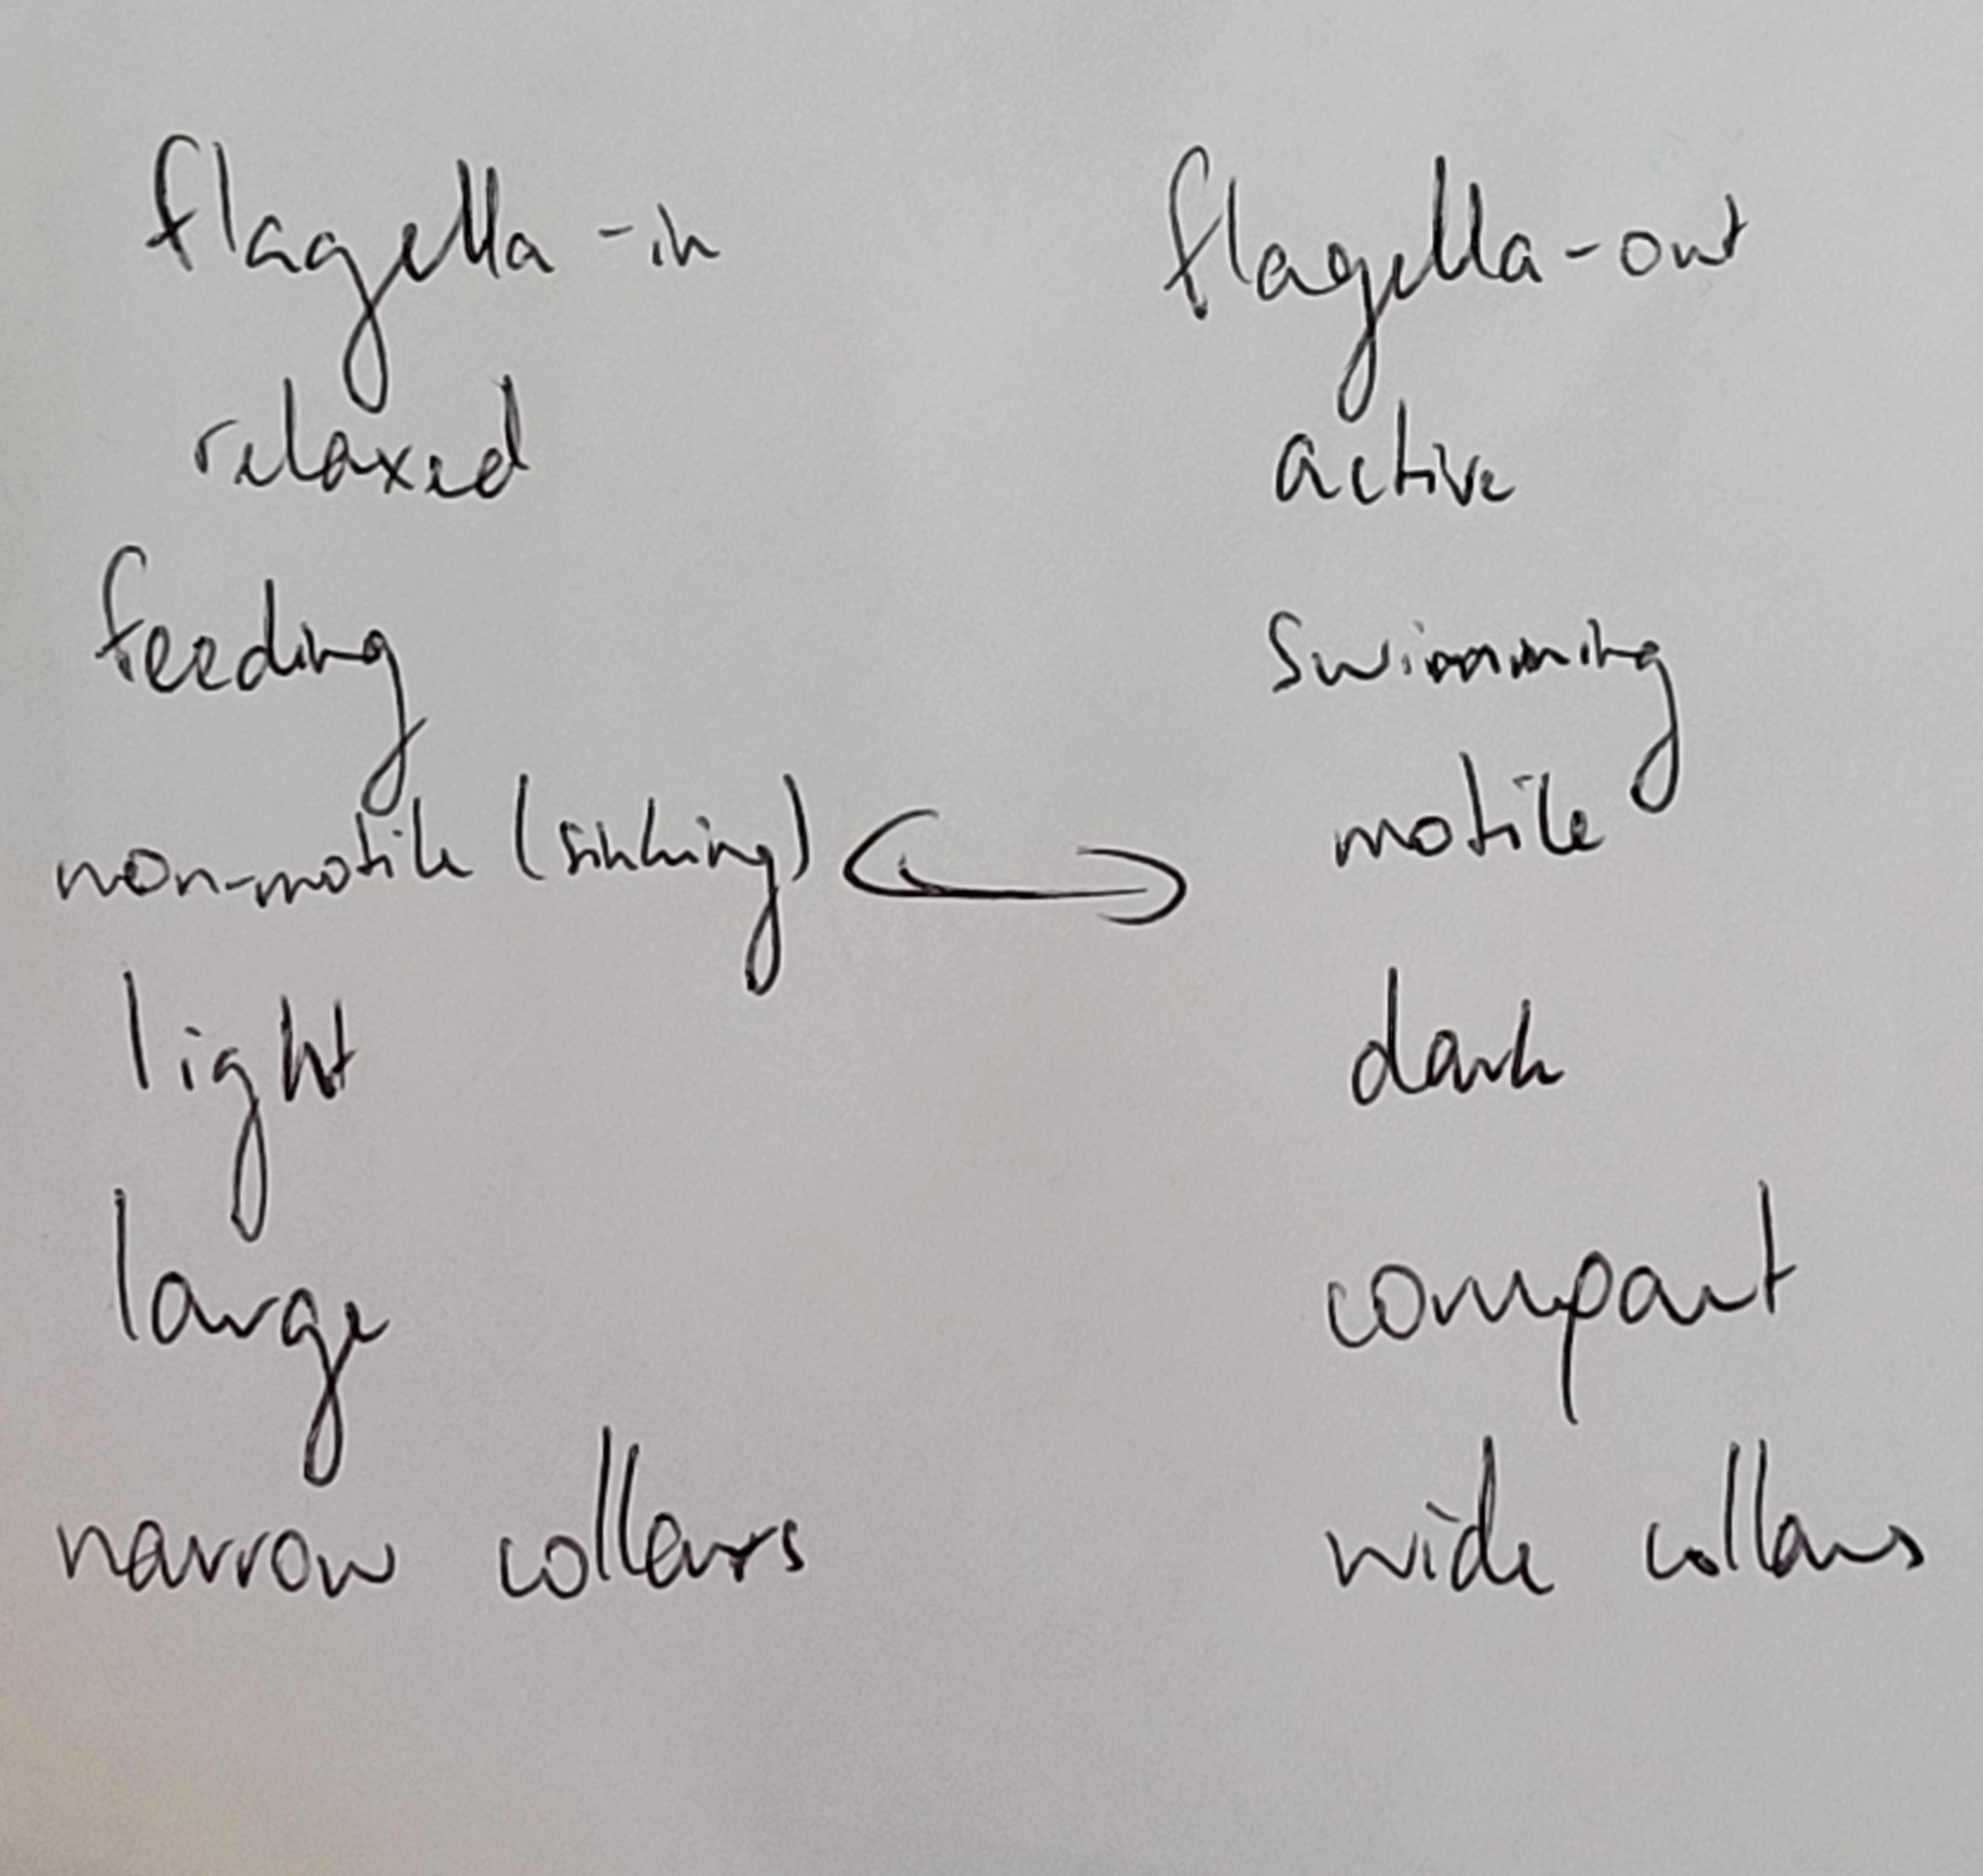
\includegraphics[width=\textwidth]{table.jpg}
		\caption{}
		\label{subfig:table}
	\end{subfigure}
	\begin{subfigure}[b]{0.4\textwidth}
		\centering
		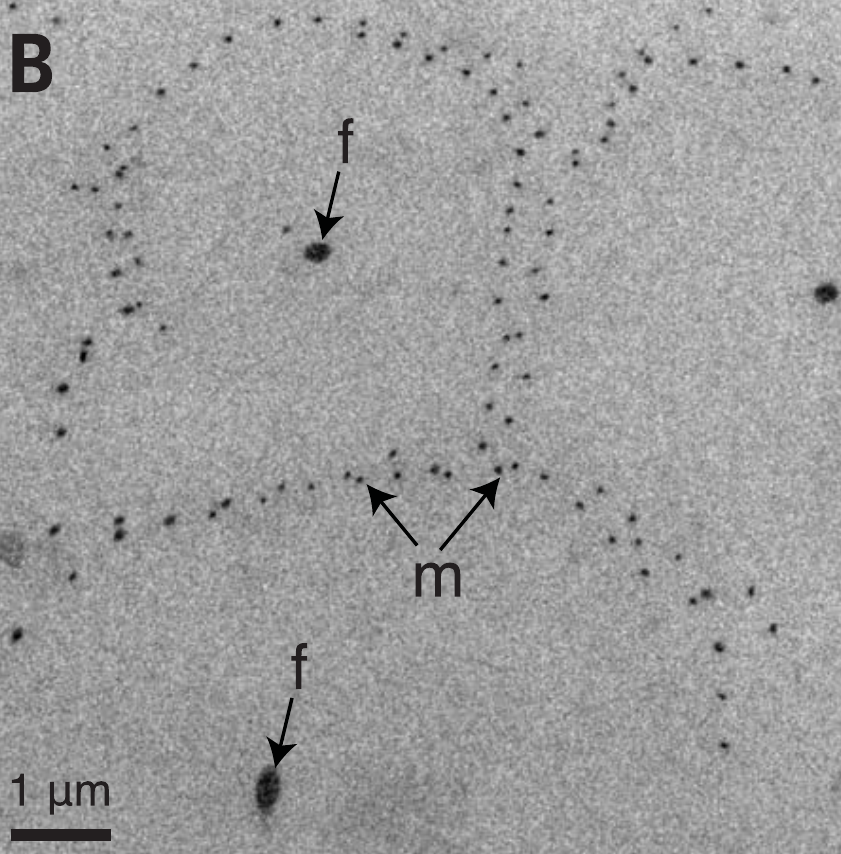
\includegraphics[width=\textwidth]{voronoi.png}
		\caption{}
		\label{subfig:voronoi}
	\end{subfigure}
	\caption[Overview of \textit{C. flexa} colonies of collared choanoflagellate cells]{Overview of \textit{C. flexa} colonies of collared choanoflagellate cells. (\ref{subfig:cflexa}) Images of the two conformations observed, flagella-in and flagella out. (\ref{subfig:table}) Summary of the two states of \textit{C. flexa} colonies. The transition from flagella-in to flagella-out is induced naturally by darkness, and the reverse transition is induced by the reintroduction of light \citep{brunet2019}. (\ref{subfig:voronoi}) Transmission electron micrograph of collar interactions between neighboring cells. f: flagella, m: microvilli. A similar figure is presented in \citet{leadbeater1983} for \textit{C. perplexa}. \cref{subfig:cflexa,subfig:voronoi} from \citet{brunet2019}. Reprinted with permission from AAAS.}
	\label{fig:cflexa}
\end{figure} 

% dynamics
Sheet inversion is rapid and reversible, allowing colonies the flexibility to convert when given suitable environmental cues.
\mynote{discuss how larger sheets are harder to invert}


Coordinated geometric changes in multicellular organisms are frequent, though they are typically achieved with several differentiated cell types or molecular signalling cascades \citep{todo}. 

\section{Motivation and objective}

As in the other basal model organisms used to probe the evolution of multicellularity, \textit{C. flexa} provides a context to study the earliest driving factors towards multicellular shape change through cooperative individual action. 
In addition to sharing similar geometry with sponge choanocyte chambers and directly informing structural modeling there \citep{asadzadeh2019}, \textit{C. flexa} captures the close relationship between geometry and flow in biological settings. 

\mynote{add here}

\section{Thesis overview}

\textit{C. flexa} provides an opportunity to study geometric changes through a simple, uncoordinated mechanism in an evolutionarily basal context. 
In this thesis, I present several approaches for modeling \textit{C. flexa} colony sheets from a mechanics perspective. 
I discuss relevant models from continuous mechanics and find that the simultaneous stretching and compression in several collar microvilli must be taken into account to appropriately model shape and dynamics. 
I review shape equations derived from variation of surface energies defined in terms of curvatures and derive an energy function for a continuous description of \textit{C. flexa} sheets. 

Due to the complexity of the continuous model, I develop a more tractable discrete model based on lessons from the continuous description. 
Collar microvilli are simplified from filaments to elastic rods, which permits a simple energy function to be defined in terms quadratic potentials on cell-collar distances and angles defined by connecting cells and collars.
The model consists of two parameters: equilibrium angles $\phi_0$ (preferred angle from the collar base to the apicobasal axis) and $\psi_0$ (preferred collar-collar contact angle). 
I take the gradient of the energy with respect to cell and collar coordinate vectors as well as the apicobasal axis vectors of all cells to solve the forces acting on all free variables in the system.
I numerically intergrate the forces on all spatial coordinates and torques on cell axes to study dynamics of cell sheets and study their mechanical equilibria.

My discrete model for \textit{C. flexa} colonies successfully models inversion in small sheets consisting of few cells. 
In larger sheets, conformational changes are hindered by rings of cells which cannot undergo the requisite stretching or compression required for inversion or folding. 
For sheets with too many cells at the boundary, the inability to compress results in buckling at the edges. 
When sheets are already curved with flagella pointing in or out, the inability to sufficiently stretch at the boundary prevents sheets from inverting and causes the cells on the sheet interior to experience substantial stress.
By framing my discrete model of \textit{C. flexa} using graph theory, I identify that the topology of the cell-cell connection network determines a sheet's ability to bend without buckling or overstretching.
This finding and my structural results compare well with the understanding of geometric effects of topological defects in crystal lattices.

The model I present makes it possible to identify regions where equilibrium angles $\phi_0$ and $\psi_0$ give minimal energy structures in the flagella-in and -out conformations.
For values that facilitate a flagella-out structure, the flagella-out structure is lower in energy than the flagella-in structure when sheet size prevents inversion as expected.
I argue that the greater amount of time required for larger sheets to invert is the result of a larger energetic barrier or smaller net internal forces, rather than greater hydrodynamic damping through drag. 
This effect from topological constraints at the sheet boundary explains the rapid contraction and slow inversion observed in large sheets in \citet{brunet2019}.
My model supports the hypothesis that \textit{C. flexa} sheets are able to invert as a result of extreme stretching at sheet boundaries or topological changes through collar-collar linkages temporarily breaking.
